\documentclass[10pt,a4paper]{article}
\usepackage[utf8]{inputenc}

% \usepackage{ngerman}  % german documents
\usepackage{graphicx}  % import graphics einbinden
\usepackage{listings}  % support source code listing
\usepackage{amsmath}  % math stuff
\usepackage{amssymb} % 
\usepackage{a4wide} % wide pages
\usepackage{fancyhdr} % nice headers
\usepackage{float}
\usepackage{longtable}
\lstset{basicstyle=\footnotesize,language=Python,breaklines=true,numbers=left, numberstyle=\tiny, stepnumber=5,firstnumber=0, numbersep=5pt} % set up listings
\pagestyle{fancy}             % header
\setlength{\parindent}{0pt}   % no indentation

\usepackage[pdfpagemode=None, colorlinks=true,  % url coloring
           linkcolor=blue, urlcolor=blue, citecolor=blue, plainpages=false, 
           pdfpagelabels,unicode]{hyperref}
           
% change enums style: first level (a), (b), (c)           
\renewcommand{\labelenumi}{(\alph{enumi})}
\renewcommand{\labelenumii}{(\arabic{enumii})}

%lecture name
\newcommand{\lecture}{
	Bioinformatics III
}           

%assignment iteration
\newcommand{\assignment}{
	Third Assignment
}


%set up names, matricle number, and email
\newcommand{\authors}{
  \begin{tabular}{rl}
    \href{mailto:s8tbscho@stud.uni-saarland.de}{Thibault Schowing} & (2571837)\\
    \href{mailto:wiebkeschmitt@outlook.de}{Wiebke Schmitt} & (2543675)
  \end{tabular}
}

% use to start a new exercise
\newcommand{\exercise}[1]
{
  \stepcounter{subsection}
  \subsection*{Exercise \thesubsection: #1}

}

\begin{document}
\title{\Large \lecture \\ \textbf{\normalsize \assignment}}
\author{\authors}

\setlength \headheight{25pt}
\fancyhead[R]{\begin{tabular}{r}\lecture \\ \assignment \end{tabular}}
\fancyhead[L]{\authors}


\setcounter{section}{3} % modify for later sheets, i.e. 2, 3, ...
%\section{Introduction to Python and some Network Properties} % optional, note that section invocation sets the section counter + 1, so adapt the setcounter command
\maketitle

%WIEBKE !!! READ THIS !!! 
% Usefull with Latex and maths: a list of the symbols ! https://reu.dimacs.rutgers.edu/Symbols.pdf

%EXERCICE 1
\exercise{}
\begin{enumerate}

% A
\item \textit{Given the states of the features, you want to infer if two proteins are likely to physically
	interact. In practice, log-likelihood ratios are used in binary classification:}\\

\[ 
	log\frac{P(C|S)}{P(\bar{C}|S)} 
\]

\textit{Derive a term that uses observable probabilities such as $ P(S_i|C) $ to calculate the loglikelihood
	ratio from training data. How does the actual classification work?}\\



First we have: 

\[ P(S_i | C) = \frac{P(C|S_i)P(S_i)}{P(C)} \]

And: 

\[ P(S_i | \bar{C}) = \frac{P(\bar{C}|S_i)P(S_i)}{P(\bar{C})} \]

Then we develop the desired final output

\[ \frac{P(S_i|C)}{P(S_i |\bar{C})}  \Longleftrightarrow \frac{P(S_i | C)P(C)}{P(S_i |\bar{C})P(\bar{C})} = \frac{P(C|S_i)P(S_i)}{P(\bar{C}|S_i)P(S_i)} = \frac{P(C|S_i )}{P(\bar{C}|S_i)}\]



\[ log\frac{P(C|S)}{P(\bar{C}|S)} = log \prod_{i}^{n} \frac{P(S_i | C)P(C)}{P(S_i |\bar{C})P(\bar{C})} = \sum_{i}^{n} log \frac{P(S_i | C)P(C)}{P(S_i |\bar{C})P(\bar{C})} = \Lambda(C|S) \]

\[ O(C|S) =  \Lambda(C|S) O(C)\]

The posterior odd is calculated by the odds of an event ($ \frac{p(event)}{1-p(event)}$) multiplied by the likelihood of that event\footnote{Slides V4 - 4}. \\

To do the classification, we must interate through the data and calculate all the priors and likelihood. The prior $P(C)$ is made from an educated guess 
%TODO understand and complete


% B
\item \textit{Shortly discuss: What are the practical advantages of the logarithm and the likelihood ratio
	within this framework? State two reasons why this particular type of classifier may perform
	poorly on a real world dataset.}\\

% https://academic.oup.com/aje/article/153/12/1222/124010
% http://slideplayer.com/slide/5178261/
The logarithm increase is a monotonically increasing function of $x$ hence, for any positive value the maximum value of a function $f(x)$, the maximum of $f(x)$ is equal to the maximum of $log(f(x))$. This simplifies the calculation because we don't need the second derivative. A likelihood function is not concave but the log-likelihood is. Also, as seen in part A, with the log-likelihood we can turn a log of products into a sum of logs. The main inconvenient is that this method assume that all the features are independent and do not take in account the eventual correlations between them. 




% C
\newpage
\item \textit{Use the file training1.tsv to build a model. This basically means to determine all necessary
	priors and likelihoods from part (a). The file layout is explained in README.txt. Report
	$P(C)$ and $P(\bar{C})$ as well as the ten $S_i$ (feature number, variant and log-ratio) with the highest
	absolute log-likelihood ratios. Examine and comment on the results of the training-phase.
	Which features seem to be the most helpful?
}\\

Prior probability $P(C) = 0.78$\\
Prior probability $P(\bar{C}) = 0.22$\\

 



\begin{table}[H]
	\centering
	\caption{10 $S_i$ with the highest absolute log-likelihood ratio}
	\label{10most}
	\begin{tabular}{lll}
		33 & 0 & -3.7214026458194964 \\
		11 & 3 & -2.565631943311438  \\
		87 & 1 & -2.4686396773241284 \\
		53 & 1 & -2.3351082846996056 \\
		99 & 1 & -2.3061207478263537 \\
		59 & 1 & -2.2779498708596573 \\
		80 & 2 & -2.2779498708596573 \\
		86 & 3 & -2.2550655770260692 \\
		91 & 3 & -2.2173252490432223 \\
		97 & 1 & -2.2099451417455995
	\end{tabular}
\end{table}


%TODO explain 


\lstinputlisting[label=ex2-b, caption={bayes.py}] {../Scripts/bayes.py}


\end{enumerate}


% NEW EXERCICE
\newpage
\exercise{Classify real-world network examples}
\begin{enumerate}
	\item \textit{If one of the nodes has a degree of 1, then $\tilde{C}_{i,j}^{(3)} $ is infinite. What is the maximal finite value that the edge-clustering coefficient can take? For which configuration does this occur? Give an example!}
	
	The edge-clustering coefficient cannot be more than 2. In the layout below we see that the clustering coefficient for the link between node 2 and 3 is equal to $\tilde{C}_{2,3}^{(3)} = \frac{1 + 1}{min(2 - 1, 6 - 1)} = \frac{2}{1}$. We see that no matter the degree of node 3, if we connect more node to node 2 the coefficient will decrease even if the number of possible triplet increase. 
	
	
\begin{figure}[H]
	\centering
	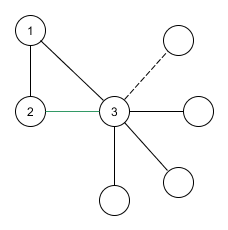
\includegraphics[width=0.5\linewidth]{expl}
	\caption{}
	\label{fig:expl}
\end{figure}
	
	
	\item (1)\textit{Give the links that you deleted from the network in (iii) by printing the names of the
		two nodes and their current edge-clustering coefficient in the order of their deletion. Of
		course, add the output to the PDF/sheet that you hand in. Implement this part as a
		script or class-based, there are no specifications you need to adjust to.}
	
	\begin{table}[H]
		\centering
		\caption{Output - Order of removed links}
		\label{table_links}
		\begin{tabular}{lll}
			Tyrion  & Sansa    & 0.33$\bar{3}$  \\
			Joffrey & Hound    & 0.5    \\
			Eddard  & Robert   & 0.5                 \\
			Eddard  & Jon      & 0.5                 \\
			Joffrey & Jaime    & 1.0                 \\
			Hound   & Mountain & 1.0                 \\
			Cersei  & Tyrion   & 1.0                 \\
			Jaime   & Cersei   & 1.0                 \\
			Catelyn & Baelish  & 1.0                 \\
			Sansa   & Baelish  & 1.0                 \\
			Eddard  & Catelyn  & 1.5                 \\
			Sansa   & Arya     & 1.5                 \\
			Eddard  & Sansa    & 1.0                 \\
			Catelyn & Arya     & 1.0                 \\
			Joffrey & Cersei   & 2.0                 \\
			Cersei  & Robert   & 1.0                 \\
			Samwell & Jon      & 2.0                 \\
			Joffrey & Robert   & $\infty$ \\
			Shae    & Tyrion   & $\infty$ \\
			Eddard  & Arya     & $\infty$ \\
			Hound   & Arya     & $\infty$ \\
			Varys   & Baelish  & $\infty$ \\
			Jaime   & Tyrion   & $\infty$ \\
			Cersei  & Mountain & $\infty$ \\
			Catelyn & Sansa    & $\infty$ \\
			Samwell & Jeor     & $\infty$ \\
			Jon     & Jeor     & $\infty$
		\end{tabular}
	\end{table}
	
	Implementation of the network decomposition:  
	
	\lstinputlisting[label=exnet-b, caption={testNetwork.py: decompose the network, output in table \ref{table_links}}] {../Scripts/part2/testNetwork.py}
	
	Implementation of the other classes. New functions have been added directly in the Network classes. 
	
	\lstinputlisting[label=exnet-b, caption={Node.py}] {../Scripts/part2/Node.py}
	\lstinputlisting[label=exnet-b, caption={AbstractNetwork.py}] {../Scripts/part2/AbstractNetwork.py}
	\lstinputlisting[label=exnet-b, caption={GenericNetwork.py}] {../Scripts/part2/GenericNetwork.py}
	
	(2) \textit{Use the links deleted in (1) in reverse order, i.e., the link that was deleted last is now
		used first to construct the communities.}
	
\begin{table}[H]
	\centering
	\caption{Inclusion of links, "x" means two subgraphs have been merged.}
	\label{tabitab}
	\begin{tabular}{|l|l|l|}
		\hline
		Link              & Merge & Graph                                                                                                                                                                                                                                                                                                                                                                                                                                                                                                \\ \hline
		Jon - Jeor        &       & {[}(Jon - Jeor){]}                                                                                                                                                                                                                                                                                                                                                                                                                                                                                   \\ \hline
		Samwell - Jeor    &       & {[}(Jon - Jeor),(Samwell - Jeor){]}                                                                                                                                                                                                                                                                                                                                                                                                                                                                  \\ \hline
		Catelyn - Sansa   &       & {[}(Catelyn - Sansa){]}                                                                                                                                                                                                                                                                                                                                                                                                                                                                              \\ \hline
		Cersei - Mountain &       & {[}(Cersei - Mountain){]}                                                                                                                                                                                                                                                                                                                                                                                                                                                                            \\ \hline
		Jaime - Tyrion    &       & {[}(Jaime - Tyrion){]}                                                                                                                                                                                                                                                                                                                                                                                                                                                                               \\ \hline
		Varys - Baelish   &       & {[}(Varys - Baelish){]}                                                                                                                                                                                                                                                                                                                                                                                                                                                                              \\ \hline
		Hound - Arya      &       & {[}(Hound - Arya){]}                                                                                                                                                                                                                                                                                                                                                                                                                                                                                 \\ \hline
		Eddard - Arya     &       & {[}(Hound - Arya),(Eddard - Arya){]}                                                                                                                                                                                                                                                                                                                                                                                                                                                                 \\ \hline
		Shae - Tyrion     &       & {[}(Jaime - Tyrion),(Shae - Tyrion){]}                                                                                                                                                                                                                                                                                                                                                                                                                                                               \\ \hline
		Joffrey - Robert  &       & {[}(Joffrey - Robert){]}                                                                                                                                                                                                                                                                                                                                                                                                                                                                             \\ \hline
		Samwell - Jon     &       & {[}(Jon - Jeor),(Samwell - Jeor),(Samwell - Jon){]}                                                                                                                                                                                                                                                                                                                                                                                                                                                  \\ \hline
		Cersei - Robert   & x     & {[}(Cersei - Mountain),(Joffrey - Robert), (Cersei - Robert){]}                                                                                                                                                                                                                                                                                                                                                                                                                                      \\ \hline
		Joffrey - Cersei  &       & \begin{tabular}[c]{@{}l@{}}{[}(Cersei - Mountain),(Joffrey - Robert), (Cersei - Robert),\\ (Joffrey - Cersei){]}\end{tabular}                                                                                                                                                                                                                                                                                                                                                                        \\ \hline
		Catelyn - Arya    & x     & \begin{tabular}[c]{@{}l@{}}{[}(Catelyn - Sansa),(Hound - Arya),(Eddard - Arya),\\ (Catelyn - Arya){]}\end{tabular}                                                                                                                                                                                                                                                                                                                                                                                   \\ \hline
		Eddard - Sansa    &       & \begin{tabular}[c]{@{}l@{}}{[}(Catelyn - Sansa),(Hound - Arya),(Eddard - Arya),\\ (Catelyn - Arya),(Eddard - Sansa){]}\end{tabular}                                                                                                                                                                                                                                                                                                                                                                  \\ \hline
		Sansa - Arya      &       & \begin{tabular}[c]{@{}l@{}}{[}(Catelyn - Sansa),(Hound - Arya),(Eddard - Arya),\\ (Catelyn - Arya),(Eddard - Sansa),(Sansa - Arya){]}\end{tabular}                                                                                                                                                                                                                                                                                                                                                   \\ \hline
		Eddard - Catelyn  &       & \begin{tabular}[c]{@{}l@{}}{[}(Catelyn - Sansa),(Hound - Arya),(Eddard - Arya),(Catelyn - Arya),\\ (Eddard - Sansa),(Sansa - Arya),(Eddard - Catelyn){]}\end{tabular}                                                                                                                                                                                                                                                                                                                                \\ \hline
		Sansa - Baelish   & x     & \begin{tabular}[c]{@{}l@{}}{[}(Varys - Baelish),(Sansa - Baelish),(Catelyn - Sansa),\\ (Hound - Arya),(Eddard - Arya),(Catelyn - Arya),\\ (Eddard - Sansa),(Sansa - Arya),(Eddard - Catelyn){]}\end{tabular}                                                                                                                                                                                                                                                                                         \\ \hline
		Catelyn - Baelish &       & \begin{tabular}[c]{@{}l@{}}{[}(Varys - Baelish),(Sansa - Baelish),(Catelyn - Sansa),\\ (Hound - Arya),(Eddard - Arya),(Catelyn - Arya),\\ (Eddard - Sansa),(Sansa - Arya),(Eddard - Catelyn),\\ (Catelyn - Baelish){]}\end{tabular}                                                                                                                                                                                                                                                                  \\ \hline
		Jaime - Cersei    & x     & \begin{tabular}[c]{@{}l@{}}{[}(Jaime - Tyrion),(Shae - Tyrion),(Cersei - Mountain),\\ (Joffrey - Robert), (Cersei - Robert),(Joffrey - Cersei){]}\end{tabular}                                                                                                                                                                                                                                                                                                                                       \\ \hline
		Cersei - Tyrion   &       & \begin{tabular}[c]{@{}l@{}}{[}(Jaime - Tyrion),(Shae - Tyrion),(Cersei - Mountain),\\ (Joffrey - Robert), (Cersei - Robert),(Joffrey - Cersei),\\ (Cersei - Tyrion){]}\end{tabular}                                                                                                                                                                                                                                                                                                                  \\ \hline
		
		
			\end{tabular}
	\end{table}

\begin{table}[H]
	\centering
	\begin{tabular}{|l|l|l|}
		\hline
		Link              & Merge & Graph                                                                                                                                                                                                                                                                                                                                                                                                                                                                                                \\ \hline

		Hound - Mountain  & x     & \begin{tabular}[c]{@{}l@{}}{[}(Varys - Baelish),(Sansa - Baelish),(Catelyn - Sansa),\\ (Hound - Arya),(Eddard - Arya),(Catelyn - Arya),\\ (Eddard - Sansa),(Sansa - Arya),(Eddard - Catelyn),\\ (Catelyn - Baelish),(Jaime - Tyrion),(Shae - Tyrion),\\ (Cersei - Mountain),(Joffrey - Robert), (Cersei - Robert),\\ (Joffrey - Cersei),(Cersei - Tyrion){]}\end{tabular}                                                                                                                            \\ \hline
		Joffrey - Jaime   &       & \begin{tabular}[c]{@{}l@{}}{[}(Varys - Baelish),(Sansa - Baelish),(Catelyn - Sansa),\\ (Hound - Arya),(Eddard - Arya),(Catelyn - Arya),\\ (Eddard - Sansa),(Sansa - Arya),(Eddard - Catelyn),\\ (Catelyn - Baelish),(Jaime - Tyrion),(Shae - Tyrion),\\ (Cersei - Mountain),(Joffrey - Robert), (Cersei - Robert),\\ (Joffrey - Cersei),(Cersei - Tyrion),(Joffrey - Jaime){]}\end{tabular}                                                                                                          \\ \hline
		Eddard - Jon      & x     & \begin{tabular}[c]{@{}l@{}}{[}(Varys - Baelish),(Sansa - Baelish),(Catelyn - Sansa),\\ (Hound - Arya),(Eddard - Arya),(Catelyn - Arya),\\ (Eddard - Sansa),(Sansa - Arya),(Eddard - Catelyn),\\ (Catelyn - Baelish),(Jaime - Tyrion),(Shae - Tyrion),\\ (Cersei - Mountain),(Joffrey - Robert), (Cersei - Robert),\\ (Joffrey - Cersei),(Cersei - Tyrion),(Joffrey - Jaime),\\ (Jon - Jeor),(Samwell - Jeor),(Samwell - Jon){]}\end{tabular}                                                         \\ \hline
		Eddard - Robert   &       & \begin{tabular}[c]{@{}l@{}}{[}(Varys - Baelish),(Sansa - Baelish),(Catelyn - Sansa),\\ (Hound - Arya),(Eddard - Arya),(Catelyn - Arya),\\ (Eddard - Sansa),(Sansa - Arya),(Eddard - Catelyn),\\ (Catelyn - Baelish),(Jaime - Tyrion),(Shae - Tyrion),\\ (Cersei - Mountain),(Joffrey - Robert), (Cersei - Robert),\\ (Joffrey - Cersei),(Cersei - Tyrion),(Joffrey - Jaime),\\ (Jon - Jeor),(Samwell - Jeor),(Samwell - Jon),\\ (Eddard - Robert){]}\end{tabular}                                    \\ \hline
		Joffrey - Hound   &       & \begin{tabular}[c]{@{}l@{}}{[}(Varys - Baelish),(Sansa - Baelish),(Catelyn - Sansa),\\ (Hound - Arya),(Eddard - Arya),(Catelyn - Arya),\\ (Eddard - Sansa),(Sansa - Arya),(Eddard - Catelyn),\\ (Catelyn - Baelish),(Jaime - Tyrion),(Shae - Tyrion),\\ (Cersei - Mountain),(Joffrey - Robert), (Cersei - Robert),\\ (Joffrey - Cersei),(Cersei - Tyrion),(Joffrey - Jaime),\\ (Jon - Jeor),(Samwell - Jeor),(Samwell - Jon),\\ (Eddard - Robert),(Joffrey - Hound){]}\end{tabular}                  \\ \hline
		Tyrion - Sansa    &       & \begin{tabular}[c]{@{}l@{}}{[}(Varys - Baelish),(Sansa - Baelish),(Catelyn - Sansa),\\ (Hound - Arya),(Eddard - Arya),(Catelyn - Arya),\\ (Eddard - Sansa),(Sansa - Arya),(Eddard - Catelyn),\\ (Catelyn - Baelish),(Jaime - Tyrion),(Shae - Tyrion),\\ (Cersei - Mountain),(Joffrey - Robert), (Cersei - Robert),\\ (Joffrey - Cersei),(Cersei - Tyrion),(Joffrey - Jaime),\\ (Jon - Jeor),(Samwell - Jeor),(Samwell - Jon),\\ (Eddard - Robert),(Joffrey - Hound),(Tyrion - Sansa){]}\end{tabular} \\ \hline
	\end{tabular}
\end{table}

%TODO draw dendogram, include listings


\begin{figure}[H]
	\centering
	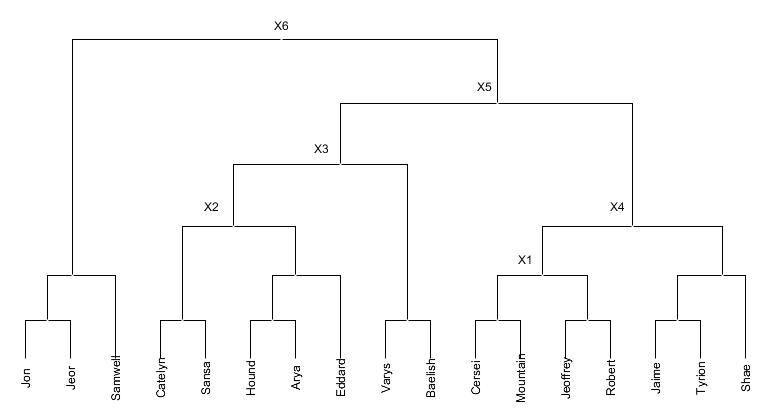
\includegraphics[width=0.9\linewidth]{dendogram}
	\caption{Dendogram}
	\label{fig:dendogram}
\end{figure}

\item Visualisation of the communities

\begin{figure}[H]
	\centering
	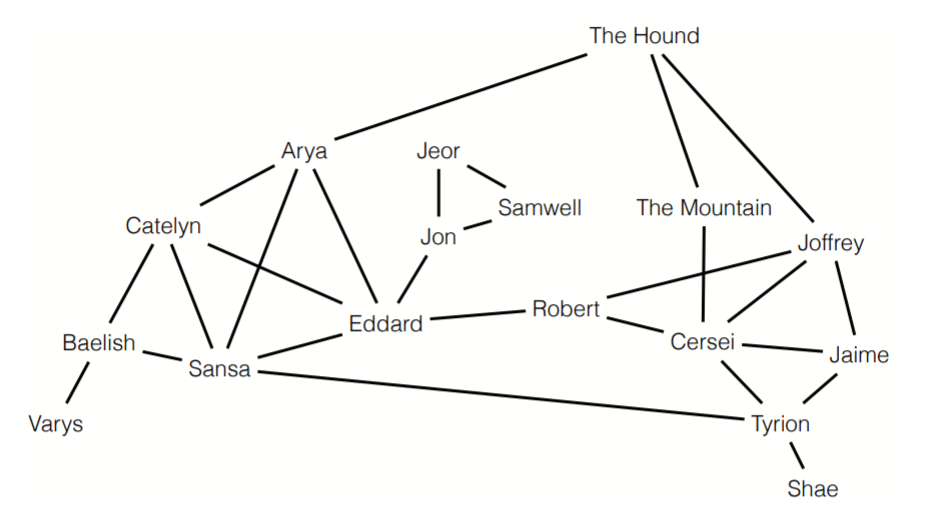
\includegraphics[width=0.7\linewidth]{viz}
	\caption{Visualisation of the network}
	\label{fig:viz}
\end{figure}

Here we can identify many communities. The two biggest are the ones we can have by separating the network in the middle ( Sansa / Tyrion, Robert / Eddard, The Hound / Arya). All the nodes have more links inside the communities than outside. 

\begin{table}[H]
	\centering
	\caption{The two big communities of the network. }
	\label{my-borness}
	\begin{tabular}{|l|l|l|}
		\hline
		Node      & $k_{in}$ & $k_{out}$ \\ \hline
		Arya      & 3        & 1         \\ \hline
		Eddard    & 3        & 1         \\ \hline
		Sansa     & 3        & 1         \\ \hline
		The Hound & 2        & 1         \\ \hline
		Robert    & 2        & 1         \\ \hline
		Tyrion    & 3        & 1         \\ \hline
	\end{tabular}
\end{table}

Here is two disjointed examples: 

\begin{table}[H]
	\centering
	\caption{Stark community. Each member have a $k_{in}$ bigger than the $k_{out}$ so the strong criterion applies. }
	\label{my-asdf}
	\begin{tabular}{|l|l|l|}
		\hline
		\textbf{Node}    & $k_{in}$ & $k_{out}$ \\ \hline
		Catelyn & 3        & 1         \\ \hline
		Arya    & 3        & 1         \\ \hline
		Eddard  & 3        & 2         \\ \hline
		Sansa   & 3        & 2         \\ \hline
	\end{tabular}
\end{table}

\begin{table}[H]
	\centering
	\caption{Jon's community, the strong criterion applies too. }
	\label{my-label}
	\begin{tabular}{|l|l|l|}
		\hline
		Node    & $k_{in}$ & $k_{out}$ \\ \hline
		Jon     & 2        & 1         \\ \hline
		Jeor    & 2        & 0         \\ \hline
		Samwell & 2        & 0         \\ \hline
	\end{tabular}
\end{table}

\end{enumerate}

\end{document}